\documentclass[border=10pt]{standalone}
\usepackage{pgfplots}
\usepgfplotslibrary{fillbetween}
\pgfplotsset{compat=1.18}
\begin{document}
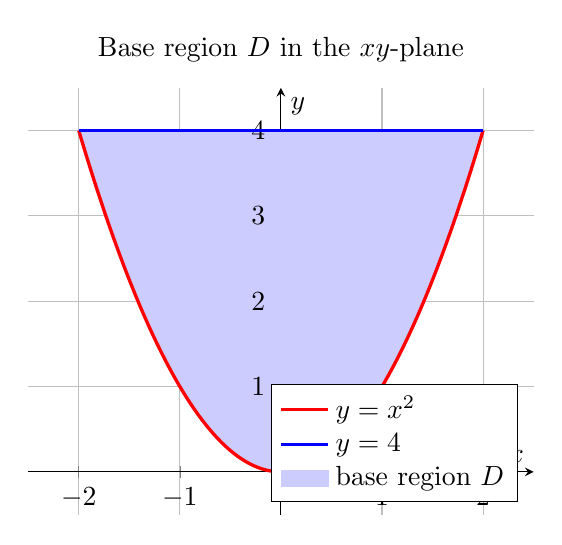
\begin{tikzpicture}
\begin{axis}[
    width=8cm, height=7cm,
    xlabel=$x$, ylabel=$y$,
    xmin=-2.5, xmax=2.5,
    ymin=-0.5, ymax=4.5,
    axis lines=middle,
    grid=both,
    title={Base region $D$ in the $xy$-plane},
    legend pos=south east,
    legend cell align=left,
]
\addplot[name path=A, domain=-2:2, samples=200, red, very thick] {x^2};
\addlegendentry{$y=x^2$}
\addplot[name path=B, domain=-2:2, samples=2, blue, very thick] {4};
\addlegendentry{$y=4$}
\addplot[blue!20] fill between[of=A and B];
\addlegendentry{base region $D$}
\end{axis}
\end{tikzpicture}
\end{document}